\documentclass[a4paper, 11pt]{article}
\usepackage[utf8]{inputenc}
\usepackage{mathtools}
\usepackage{amsmath}
\usepackage{amssymb}
\usepackage{xfrac}
\usepackage{tikz}
\usepackage{subcaption}
\usepackage{pgfplots}
\usepackage{soul}
\usepackage[margin=3cm, footskip=1cm]{geometry}
\usepackage{hyperref}
\usepackage[superscript]{cite}
\usepackage[title, titletoc]{appendix}
\usepackage[nottoc]{tocbibind}
\setlength{\belowcaptionskip}{-4pt}

\pgfplotsset{compat=1.15}

\begin{document}

\newcommand{\HRule}[1]{\rule{\linewidth}{#1}}

\begin{titlepage}
	\centering
	\includegraphics{images/epfl-logo.jpg}\par
	\vspace{1cm}
	\HRule{0.5pt}
	{\scshape \Large Semester project: \\ Perceptron learning through structure}
	\vspace{1cm}
    \HRule{0.5pt}
	{\Large Mariko Makhmutova\par}
	\vspace{8cm}
	{\large Supervised by Nicolas Macris\par}
	{\large Information Processing Group, EPFL \par}
	{\large Spring 2018\par}
	\vfill
\end{titlepage}

\tableofcontents

\newpage

\vspace{10cm}
\begin{abstract}

In this work, we study the variation of the information storage capacity of a simple perceptron when trained on image classifier patterns. We begin by studying properties of the perceptron learning structure as well as Cover's theorem and Gardner's results on storage capacity. Then, considering training sets composed of images that are classified on some number of features, we apply Gardner's method of evaluating storage capacity. We conclude that there is no variation in information storage capacity for the considered distributions.

\end{abstract}
\vfill

\newpage

\section{Properties of the perceptron}

\subsection{Model structure}

A perceptron is a layered feed-forward neural network. A connection originating from any given unit in the network can only lead to a unit in the next layer, as shown in Fig. 1.

A $K$-layer network contains a layer of input units, a layer of output units and $K-1$ layers of hidden units between them. A simple perceptron is a single-layer network with no hidden layers, as shown in Fig. 1(b). A simple perceptron with $N$-dimensional input $\xi = (\xi_1, \xi_2, ... \xi_N)$ and $M$-dimensional output $O = (O_1, ..., O_M)$ computes the output in the following way:

\begin{equation}
    O_i = g(h_i) = g \left( \sum_{j=1}^N \xi_j w_{ij} \right)
\end{equation}

The $w_{ij}$ factors are the components of the weight vector $w_i$ and $g(\cdot)$ is the activation function. $g(\cdot)$ is usually a non-linear threshold function. We will henceforth use $g(h) = \mathrm{sgn} (h)$ as our activation function.

We will not take into account any biases for simple perceptrons, as having bias element is equivalent to having an $(N+1)$-dimensional input and setting $\xi_{N+1} = -1$.

Perceptrons are used for supervised learning, that is, given a training set of $p$ input-output patterns, with input $\xi$ and output $\zeta$, we want the following to be true for every $i = 1, 2, ..., M$ and $\mu = 1, 2, ..., p$:

\begin{equation}
    O_i^\mu = \zeta_i^\mu
\end{equation}

We assume that target outputs $\zeta_i^\mu \in \{ \pm 1 \}$. Thus the problem in (2) is reduced to requiring that the signs of $h_i^\mu$ and $\zeta_i^\mu$ be the same for every $i$ and $\mu$. We suppose that output units are i.i.d., so we can drop the $i$ subscripts without loss of generality. Thus, for every $\mu$, we can reformulate (2) as:

\begin{equation}
    sgn(w \cdot \xi^\mu) = \zeta^\mu
\end{equation}

This implies that every input $\xi^\mu$ projected onto $w$ has the same sign as $\zeta^\mu$. Positive and negative projections onto $w$ are separated by the hyperplane that is perpendicular to $w$ and goes through the origin. For a perceptron to learn all the input-output patterns in the training set, this hyperplane must divide the inputs that have positive and negative targets, as shown in Fig. 2.

\begin{center}
\begin{figure}[bhtp]
    \centering
    \captionsetup{justification=centering, font=small, margin=0.5cm}
    \begin{subfigure}[b]{0.52\linewidth}
        \centering
        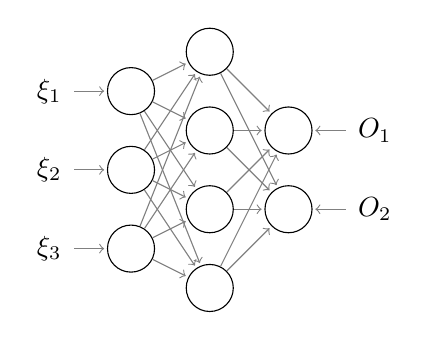
\begin{tikzpicture}[scale=1, shorten >=1pt,->,draw=black!50, node distance=1cm]
    \tikzstyle{every pin edge}=[<-,shorten <=1pt]
    \tikzstyle{neuron}=[circle,fill=black!25,minimum size=17pt,inner sep=0pt]
    \tikzstyle{input neuron}=[neuron, draw=black, fill=white!50];
    \tikzstyle{output neuron}=[neuron, draw=black, fill=white!50];
    \tikzstyle{hidden neuron}=[neuron, draw=black, fill=white!50];
    
    % Draw the input layer nodes
    \foreach \name / \y in {1,...,3}
    % This is the same as writing \foreach \name / \y in {1/1,2/2,3/3,4/4}
        \node[input neuron, pin=left:$\xi_{\y}$] (I-\name) at (0,-\y) {};

    % Draw the hidden layer nodes
    \foreach \name / \y in {1,...,4}
        \path[yshift=0.5cm]
            node[hidden neuron] (H-\name) at (1cm,-\y cm) {};
            
    % Draw the output layer node
    \node[output neuron, pin=right:$O_1$, right of=H-2] (O-1) {};
    \node[output neuron, pin=right:$O_2$, right of=H-3] (O-2) {};

    % Connect every node in the input layer with every node in the hidden layer.
    \foreach \source in {1,...,3}
        \foreach \dest in {1,...,4}
            \path (I-\source) edge (H-\dest);

    % Connect every node in the hidden layer with the output layer
    \foreach \source in {1,...,4}
        \foreach \dest in {1,...,2}
        \path (H-\source) edge (O-\dest);

\end{tikzpicture}
        \caption{Two-layer perceptron}
    \end{subfigure}
    \begin{subfigure}[b]{0.46\linewidth}
        \centering
        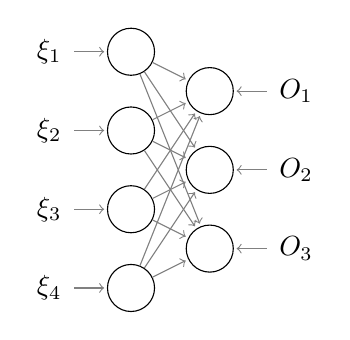
\begin{tikzpicture}[scale=1, shorten >=1pt,->,draw=black!50, node distance=1cm]
    \tikzstyle{every pin edge}=[<-,shorten <=1pt]
    \tikzstyle{neuron}=[circle,fill=black!25,minimum size=17pt,inner sep=0pt]
    \tikzstyle{input neuron}=[neuron, draw=black, fill=white!50];
    \tikzstyle{output neuron}=[neuron, draw=black, fill=white!50];
    
    % Draw the input layer nodes
    \foreach \name / \y in {1,...,4}
    % This is the same as writing \foreach \name / \y in {1/1,2/2,3/3,4/4}
        \node[input neuron, pin=left:$\xi_{\y}$] (I-\name) at (0,-\y) {};

    % Draw the hidden layer nodes
    \foreach \name / \y in {1,...,3}
        \path[yshift=-0.5cm]
            node[output neuron, pin=right:$O_\y$] (O-\name) at (1cm,-\y cm) {};
    
    % Connect every node in the input layer with every node in the hidden layer.
    \foreach \source in {1,...,4}
        \foreach \dest in {1,...,3}
            \path (I-\source) edge (O-\dest);
\end{tikzpicture}
        \caption{Simple perceptron}
    \end{subfigure}
    \caption{Examples of perceptrons}
    \label{fig:1}
\end{figure}
\end{center}

We can clearly see that the solvability of a problem by a simple perceptron depends on whether the problem is linearly separable or not. A linearly separable problem is one where there exists a hyperplane dividing the input-output patterns with output units $\zeta^\mu = -1$ from those with output units $\zeta^\mu = 1$. Since we are not working with biases, the separating hyperplane must pass through the origin. In the case of multiple units, such a hyperplane must exist for each output unit.

\begin{center}
\begin{figure}[thbp]
\centering
\captionsetup{justification=centering, font=small, margin=0.5cm}
\begin{tikzpicture}
\begin{axis}[
    axis lines=middle,
    xmin=-10, xmax=10,
    ymin=-8, ymax=8,
    xlabel=$\xi_1$, ylabel=$\xi_2$,
    xtick=\empty, ytick=\empty
]
\addplot [only marks] table {
-8 -4
-6  2
-4  5   
-3  7
-2  3
2  6
};
\addplot [only marks, mark=o] table {
-3  -5
3  -7
1  -4
5   -3
6   3
7   -1
};
\addplot [domain=-6:6, samples=2, dashed] {x};
\addplot [domain=0:2, samples=2, -stealth] {-x} node[above right] {$w$};
\end{axis}
\end{tikzpicture}
\caption{For $N=2$, output targets $\zeta^\mu$ are divided by a hyperplane perpendicular to $w$, passing through the origin. Adapted from \cite[p.93]{introbook}}
\label{fig:2}
\end{figure}
\end{center}

\subsection{Learning algorithm}

The perceptron learning algorithm is the procedure through which the perceptron finds an appropriate weight vector $w$ to satisfy (3).\footnote[1]{We assume a single output unit, but the algorithm can be easily generalized for multiple output units}

We begin with a null vector $w$. Then, iterating over the inputs $\xi_j^\mu$, we verify whether the output units correspond to the desired ones. If the output unit $O^\mu$ corresponds to the desired output unit $\zeta^\mu$, we do not change the value of the weight vector element feeding into that output unit. Otherwise, we update the weight vector as follows:

\begin{equation}
    w_{j}^{new} = w_{j}^{old} + \Delta w_{j}
\end{equation}

\noindent where:

\begin{equation}
    \Delta w_{j} = \eta (\zeta^{\mu} - O^{\mu}) \xi_j^{\mu}
\end{equation}

\noindent with $\eta \ll 1$ defined as the learning rate of the perceptron.

Taking into consideration the possibility of small errors in the input patterns, we set a requirement that the output is greater than some predefined margin $\kappa > 0$. Combining this requirement with the condition that $h^\mu$ and $\zeta^\mu$ be of the same sign, we obtain the following condition to verify when updating the weight vector:

\begin{equation}
    \zeta^\mu h^\mu \equiv \zeta^\mu \sum_j w_{j} \xi_j^\mu > N \kappa
\end{equation}

Since the left-hand side of the inequality scales with $N$, we add $N$ to the right-hand side of the inequality, allowing $\kappa$ to be constant. The derivation of $\Delta w_{j}$ thus becomes:

\begin{equation}
    \Delta w_{j} = \eta \Theta(N \kappa - \zeta^\mu h^\mu) \zeta\mu \xi_j^{\mu}
\end{equation}

\noindent where $\Theta$ denotes the step function.

Equation (7) represents the perceptron learning rule, describing the way in which a perceptron updates the weight vector as it learns new patterns.

\section{Information storage capacity}

Consider a simple perceptron with $N$-dimensional input and $M$-dimensional output. We are interested in studying the information storage capacity of such a perceptron as $N$ tends to infinity while $M$ remains fixed. The information storage capacity of a perceptron is defined as the maximum number of patterns that it can learn.

We interpret this for a simple perceptron with input vector $\xi$ and computed binary outputs $O_i$ for $i = 1, 2, ... M$. Finding the capacity is equivalent to defining a maximum $p$ value such that, given a training set of $p$ patterns $\xi_j^\mu \longrightarrow \zeta_i^\mu$ with $j = 1, 2, ..., N$ and $\mu = 1, 2, ... p$, the following relation is satisfied for all $i$ and $\mu$:

\begin{equation}
    \zeta_i^\mu = O_i^\mu
\end{equation}

We study two approaches to computing storage capacity. Cover's theorem \cite{introbook, orhan} relies on the reasoning that for a set of patterns to be stored in a neural network, the patterns must be linearly separable. Gardner's work \cite{introbook, gardner} uses replica methods to compute the capacity.

\subsection{Cover's theorem}

Suppose that we have $p$ points in $\mathbb{R}^N$. There are $2^p$ possible partitions of these $p$ points into two classes, for example colouring each point in red or blue. We define a dichotomy as a partition that yields linearly separable classes, i.e. where the red and blue points can be separated by an $(N-1)$-dimensional hyperplane. We are interested in determining how many partitions of the $p$ points yield dichotomies.

We assume that the points are in general position, so that any subset of $N$ or fewer points is linearly independent.

We denote the number of dichotomies of $p$ points in $N$ dimensions by $C(p, N)$. A detailed explanation in Appendix A describes how we obtain the following equation representing the number of dichotomies $C(p, N)$:

\begin{equation}
    C(p, N) = 2 \sum_{i=0}^{N-1} \binom{p-1}{i}
\end{equation}

Fig. 3 shows the fraction of partitions of $p$ points a simple perceptron is able to dichotomize. There is clearly a sharp phase transition with large $N$ when $p = 2N$. At this point, there is a transition from the perceptron being able to store all $p$ points to none of them. This phase transition represents the maximum capacity at $p = 2N$.

\begin{center}
\begin{figure}[thbp]
    \centering
    \captionsetup{justification=centering, font=small, margin=0.5cm}
    \includegraphics[height=6cm]{images/capacity-graph.png}
    \caption{Fraction of partitions of $p$ points that a simple perceptron is able to dichotomize for varying $N$}
\end{figure}
\end{center}

\subsection{Gardner's theory}

Gardner's approach to deducing information storage capacity evaluates the fraction of weight space in which a perceptron is able to store a given number of patterns. A more complete version of this proof can be referred to in Appendix B.

We consider a simple perceptron with $N$-dimensional binary input vector $\xi$ and $M$-dimensional binary output vector $O$ given by:

\begin{equation}
    O_i = \mathrm{sgn} \left( N^{-\sfrac{1}{2}} \sum_j w_{ij} \xi_j \right)
\end{equation}

\noindent for $i = 1, 2, ..., M$.

Suppose a training set of $p$ patterns $\xi_j^\mu \longrightarrow \zeta_i^\mu$ with $\mu = 1, 2, ... p$. It is assumed that all $\xi_j^\mu, \zeta_i^\mu$ are i.i.d. equiprobable Bernoulli random variables, such that $\xi_j^\mu, \zeta_i^\mu \in \{ \pm 1 \}$. We want to deduce in what fraction of weight space the following relation is satisfied for all $i$ and $\mu$:

\begin{equation}
    \zeta_i^\mu = O_i^\mu
\end{equation}

This condition is identical for each index $i$, so we can drop the $i$ to consider a single output unit to simplify our calculations without loss of generality. Using the definition of $O$, we rewrite the above relation as:

\begin{equation}
    \zeta_i^\mu N^{-\sfrac{1}{2}}\sum_j w_{j} \xi_j^\mu > 0
\end{equation}

Condition (12) can be strengthened by considering the possibility of small errors in the input pattern. To do so, we replace the right-hand side of the inequality with a stability parameter $\kappa > 0$. We obtain the following strengthened condition:

\begin{equation}
    \zeta^\mu N^{-\sfrac{1}{2}}\sum_j w_{j} \xi_j^\mu > \kappa
\end{equation}

We add the following constraint to the problem to keep the weight vector $w$ within bounds:

\begin{equation}
    \sum_j w_j^2 = N
\end{equation}

The principal quantity that we want to calculate is the volume fraction of weight space in which (13) is satisfied:

\begin{equation}
    V = \frac{\int \left( \prod_\mu \Theta \left( \zeta^\mu N^{-\sfrac{1}{2}}\sum_j w_{j} \xi_j^\mu - \kappa \right) \right) \delta \left( \sum_j w_j^2 - N \right) \, \mathrm{d} w}{\int \delta(\sum_j w_j^2 - N) \, \mathrm{d} w}
\end{equation}

Here, the Dirac delta function $\delta$ is used to enforce (14) and the step function $\Theta$ is used to restrict the numerator to regions of the weight space satisfying condition (13).

Applying the replica trick, and through a series of simplifications of the expected value of volume $V$, we obtain the following equation, which gives the storage capacity for fixed $\kappa$:

\begin{equation}
    \alpha_c (\kappa) = \left[ \int_{-\kappa}^\infty \frac{dt}{\sqrt{2 \pi}} e^{t^2 / 2} (t + \kappa)^2 \right] ^{-1}
\end{equation}

We observe that by setting parameter $\kappa = 0$ we obtain the results observed in Cover's theorem.

\section{Applications in image classification}

It is interesting to determine information storage capacity in relation to image classification. We are often concerned with acquiring enough data to train a model, but we should also consider the situation in which the model is unable to learn all of the patterns in the training set. In this section we will study how storage capacity varies for two different input-output pattern distributions used to represent image classifier patterns \footnote{The representations considered are inspired by an example in [\citen{mezard}].}.

We consider a training set of $p$ images, each of which contains $N$ pixels. Suppose that there is some number $R$ of features that are present in each pixel and image. We represent the input pattern for pixel $j$ of image $\mu$ by:

\begin{equation}
    \xi_j^\mu = \frac{1}{\sqrt{R}} \sum_{r=1}^R u_{j r} v_{r \mu}
\end{equation}

\noindent where $U$ is an $N \times R$ matrix representing the presence of each feature in each pixel and $V$ is an $R \times p$ matrix representing the presence of each feature in each image.

We want to perform a binary classification of each image, so we denote the output pattern for each image $\mu$ by $\zeta^\mu$, with $\zeta^\mu \in \{ \pm 1 \}$.\footnote{The training set can be generalized for multiple output dimensions, provided that they are i.i.d.}

We base our deduction of the storage capacity for the image training set described above on Gardner's work, adapting the calculations where needed.

First, we consider the case of output being independent of the input. We suppose that all elements in $U$ and $V$ are i.i.d. Bernoulli random variables with parameters $\phi$ and  $\gamma$ respectively, taking values in $\{ \pm 1 \}$. The output pattern $\zeta$ follows an equiprobable Bernoulli distribution, taking values in $\{ \pm 1 \}$.

Applying the appropriate modifications to Gardner's work, which can be referred to in detail in Appendix C, we observe that the storage capacity does not change for this training set. This implies that the maximum number of image patterns following this distribution that a perceptron is able to learn is $2N$.

We note that the results do not vary depending on the number of features $R$, nor the values of parameters $\phi$ and $\gamma$ describing the input pattern distribution.

To verify if this property can be generalized to other training sets we consider a different distribution. In this case, we suppose that the output classification uniquely depends on the presence of each feature in an image, not in each pixel. To model such a training set, we consider the a similar input pattern distribution to the one in the first case. We suppose that all elements in $U$ and $V$ are i.i.d. equiprobable Bernoulli random variables, taking values in $\{ \pm 1 \}$. The output pattern distribution is modified as such: for every pattern $\mu = 1, 2, ..., p$, we have $\zeta^\mu = f(V^\mu)$, $\zeta^\mu \in \{ \pm 1 \}$, where $f$ is a function used to classify the output.

Performing a similar calculation as we did for the previous distribution, which can be referred to in more detail in Appendix D, we conclude that the storage capacity does not change for this input-output pattern distribution. Again, the results are invariant with respect to the number of features $R$.

\section{Conclusion}
The information storage capacity of a perceptron is an important structural property, which allows us to set an upper limit on the number of patterns a perceptron is able to learn. Applying methods studied in literature, we computed the storage capacity for two training sets representing image classifiers. We observed that the storage capacity was invariant for these training sets, regardless of the number of image features considered.

Unfortunately, due to time constraint, we were unable to study other training sets, to determine a general rule for this property. It would be interesting to consider, in a further work, how the storage capacity changes with more complex input pattern distributions. Another, considerably more complex, training set to consider would be one with multiple output dimensions that are not i.i.d., to imitate a more realistic model.

\newpage

\section*{Appendix A}

\addcontentsline{toc}{section}{Appendix A}

In this section, we provide a proof to Cover's theorem, which deduces storage capacity using the argument that a training set of patterns must be linearly separable for a neural network to be able to store all of the patterns.

Suppose that we have $p$ points in $\mathbb{R}^N$. There are $2^p$ possible partitions of these $p$ points into two classes, for example colouring each point in red or blue. We call a partition that yields linearly separable classes, i.e. where the red and blue points can be separated by a $(N-1)$-dimensional hyperplane a dichotomy. We are interested in determining how many partitions of the $p$ points yield dichotomies.

We assume that the points are in general position, so that any subset of $N$ or fewer points is linearly independent.

Let us denote the number of dichotomies by $C(p, N)$. Suppose that we have $p$ linearly separable points and add a new point P. There are two possibilities of where P can be placed:

\begin{enumerate}
    \item There is a separating hyperplane for the previous $p$ points passing through P. This means that each of the dichotomies for the previous $p$ points yields two distinct dichotomies, because the hyperplane passing through P can be shifted infinitesimally to either side to change the colour of P, without affecting the colourings of any of the previous $p$ points.
    \item There is no separating hyperplane passing through P. The new point P can only have one colour for it to yield a dichotomy, so there is only one new dichotomy for each of the previous dichotomies.
\end{enumerate}

The first case corresponds to $C(p, N-1)$ dichotomies. This is because we take the same $p$ points as before and restrict the dichotomies to those that allow for a separating hyperplane to pass through a point P, which is analogous to restricting the hyperplanes to $N-1$ dimensions instead of $N$, as we can see in Fig. 5.

Thus, to calculate $C(p+1, N)$, we count the number of dichotomies in (1) twice and the number of dichotomies in (2) once. Clearly, this is the same as counting $C(p, N)$ and adding the number of dichotomies in (1).

We can write $C(p, N) = a + b$, where $a$ corresponds to the number of dichotomies in (1) and $b$ corresponds to the number of dichotomies in (2) [\citen{orhanemail}]. Thus, we have:

\begin{align}
    C(p+1, N) & = 2a + b \nonumber \\
    & = a + (a + b) \nonumber \\
    & = C(p, N-1) + C(p, N)
\end{align}

Thus, we have obtained a recurrence equation to find the number of dichotomies in function of the number of points $p$ and input-dimension $N$.

We will now deduce the numerical value of $C(p, N)$ from the recurrence equation. First, we admit that $C(1, k) = 0$ if $k < 1$. We also acknowledge that $C(1, k) = 2$ for $k \geqslant 1$, because a single point can only have two dichotomies in any number of dimensions -- one where the point is coloured red, and one where it is coloured blue.

\pagebreak

\begin{figure}[bhtp]
    \centering
    \captionsetup{justification=centering, font=small, margin=0.5cm}
    \frame{\includegraphics[height=0.25\textwidth]{images/cover-2d-example.png}}
    \caption{For $N=2$, $p=12$, we see that if a new point falls in the shaded area (case 1), it can be coloured either red or blue to create a dichotomy. If the point falls in either of the unshaded areas (case 2), it can only be one of two colours for a dichotomy to exist.}
\end{figure}

\begin{figure}[bhtp]
    \centering
    \captionsetup{justification=centering, font=small, margin=0.5cm}
    \frame{\includegraphics[height=0.25\textwidth]{images/reduce-dimension.png}}
    \caption{Limiting hyperplanes to those that pass through O and P is equivalent to projecting onto the plane perpendicular to OP, thus reducing the dimension of each hyperplane by one. \cite[p.113]{introbook}}
\end{figure}

We observe $p-1$ iterations of (18):

\begin{equation}
    \begin{split}
    C(p+1, N)
    & = C(p, N) + C(p, N-1) \\
    & = C(p-1, N) + 2 C(p-1, N-1) + C(p-1, N-2) \\
    & = \quad ... \\
    & = \binom{p}{0} C(1, N) + \binom{p}{1} C(1, N-1) + ... + \binom{p}{p} C(1, N-p) \end{split}
\end{equation}

From the above observations, we obtain the following hypothesis:

\begin{equation}
    C(p, N) = 2 \sum_{i=0}^{N-1} \binom{p-1}{i}
\end{equation}

By a verification using a proof by induction, we confirm that (20) indeed describes the number of dichotomies in function of the input dimension $N$ and the number of points $p$.

In Fig. 6, we plot the values of $p/N$ against $C(p, N)/2^p$ to see what fraction of partitions of $p$ points a simple perceptron is able to find dichotomies for. We can clearly see that there is a sharp transition with large $N$ when $p = 2N$. At this point, the simple perceptron goes from being able to store all $p$ points to none of them. By definition, this gives the information storage capacity $p_{\max}$ of a simple perceptron:

\begin{equation}
    p_{\max} = 2N
\end{equation}

\pagebreak

\begin{figure}[thbp]
    \centering
    \captionsetup{justification=centering, font=small, margin=0.5cm}
    \includegraphics[height=5cm]{images/capacity-graph.png}
    \caption{Fraction of partitions of $p$ points that a perceptron is able to dichotomize for varying values of $N$}
\end{figure}


\vspace{-0.5cm}

\section*{Appendix B}

\addcontentsline{toc}{section}{Appendix B}

In this appendix, we summarize Gardner's theory. In her work, Gardner determines the storage capacity by computing the fraction of weight space in which a perceptron is able to store a given number of patterns. 

We use a simple perceptron with $N$ binary input units $\xi_j \in \{ \pm 1 \}$ and $M$ binary output units which are calculated using $O_i = \mathrm{sgn} (N^{-\sfrac{1}{2}} \sum_j w_{ij} \xi_j)$ for $i = 1, 2, ... M$. 

Given a training set of $p$ patterns $\xi_j^\mu \longrightarrow \zeta_i^\mu$ with $\mu = 1, 2, ... p$, we want to know in what fraction of weight space the following relation is satisfied for all $i$ and $\mu$:

\begin{equation}
    \zeta_i^\mu = O_i
\end{equation}

This condition is identical for each index $i$, so we can drop the $i$ and consider the case of one output unit to simplify our calculations without loss of generality. We use the definition of $O$ to rewrite the condition as:

\begin{equation}
    \zeta^\mu N^{-\sfrac{1}{2}} \sum_j w_{j} \xi_j^\mu > 0
\end{equation}

We strengthen (23) by considering the possibility of minor errors in the input pattern. To do so, we replace the right-hand side of the equation with a stability parameter $\kappa > 0$. This gives the following strengthened condition:

\begin{equation}
    \zeta^\mu N^{-\sfrac{1}{2}}\sum_j w_{j} \xi_j^\mu > \kappa
\end{equation}

Note that the $N$ weights $w_j$ are of order 1, and a sum of $N$ terms of order 1 gives a term of order $N^{\sfrac{1}{2}}$. To prevent (24) from scaling with $N$, we add a $N^{-\sfrac{1}{2}}$ factor on the left-hand side. This allows $\kappa$ to be a constant independent of $N$.

We add the following constraint to the problem to keep the weights within bounds:

\begin{equation}
    \sum_j w_j^2 = N
\end{equation}

The principal quantity that we want to calculate is the volume fraction of weight space in which (24) is satisfied:

\begin{equation}
    V = \frac{\int \left(\prod_\mu \Theta \left( \zeta^\mu N^{-\sfrac{1}{2}} \sum_j w_{j} \xi_j^\mu - \kappa \right) \right) \delta \left( \sum_j w_j^2 - N \right) \, \mathrm{d} w}{\int \delta(\sum_j w_j^2 - N) \, \mathrm{d} w}
\end{equation}

Here, the Dirac delta function $\delta$ is enforces condition (25) and the step function $\Theta$ restricts the numerator to regions of the weight space satisfying (24).

Given that both the numerator and the denominator in (26) grow exponentially with $N$, we are interested in calculating the average of $\log (V)$, rather than of $V$ itself, which is the approximation of the following limit:

\begin{equation}
    \ln Z = \lim_{n \longrightarrow 0} \frac{Z^n - 1}{n}
\end{equation}

Using the replica trick, we compute the expected value of $V^n$ over the training set:

\begin{equation}
    \textstyle{\mathbb{E}_{\xi, \zeta} [V^n] = \frac{\mathbb{E}_{\xi, \zeta} \left [\prod_{\alpha=1}^n \int \left( \prod_\mu \Theta \left( \zeta^\mu N^{-\sfrac{1}{2}} \sum_j w_{j}^\alpha \xi_j^\mu - \kappa \right) \right) \delta \left( \sum_j (w_j^\alpha)^2 - N \right) \, \mathrm{d} w^\alpha \right] }{\Pi_{\alpha=1}^n \int \delta(\sum_j (w_j^\alpha)^2 - N) \, \mathrm{d} w^\alpha}}
\end{equation}

We proceed by simplifying (28) using integral representations of the step and delta functions.

The step function can be written in its integral form as:

\begin{equation}
    \Theta(z - \kappa) = \int_\kappa^{\infty} \delta(\lambda - z) \mathrm{d} \lambda = \int_\kappa^{\infty} \int_0^{2 \pi} \frac{1}{2\pi} e^{ix(\lambda - z)} \, \mathrm{d} x \, \mathrm{d} \lambda
\end{equation}

Since (28) has step functions for each $\alpha$ and $\mu$, we must use corresponding variables $\lambda_\alpha^\mu$, $x_\alpha^\mu$. The step function in the numerator becomes:

\begin{equation}
    \Theta \big( \zeta^\mu N^{-\sfrac{1}{2}} \sum_j w_{j}^\alpha \xi_j^\mu - \kappa \big) = \frac{1}{2\pi}\int_\kappa^{\infty} \int_0^{2 \pi} e^{ix_\alpha^\mu\lambda_\alpha^\mu} e^{-ix_\alpha^\mu z_\alpha^\mu} \, \mathrm{d} x_\alpha^\mu \, \mathrm{d} \lambda_\alpha^\mu
\end{equation}

\noindent where $z_\alpha^\mu = \zeta^\mu N^{-\sfrac{1}{2}} \sum_j w_{j}^\alpha \xi_j^\mu$.

We can easily compute the expected value over the $\xi_j^\mu$'s and $\zeta^\mu$'s, since they only appear in the last factor of (30).

Under the hypothesis that the input and output patterns are i.i.d. equiprobable Bernoulli random variables, we have:

\begin{align}
    \mathbb{E} \Big[ \prod_{\mu\alpha} e^{-ix_\alpha^\mu z_\alpha^\mu} \Big]
    &= \prod_{j\mu} \mathbb{E} \big[ \exp(-i\zeta^\mu \xi_j^\mu N^{-\sfrac{1}{2}} \sum_\alpha x_\alpha^\mu w_{j}^\alpha) \big] \nonumber \\
    &= \prod_{j\mu} \big( \frac{1}{2}\exp(-iN^{-\sfrac{1}{2}} \sum_\alpha x_\alpha^\mu w_{j}^\alpha) + \frac{1}{2} \exp(iN^{-\sfrac{1}{2}} \sum_\alpha x_\alpha^\mu w_{j}^\alpha) \big) \nonumber \\
    &= \prod_{j\mu} \cos \big( N^{-\sfrac{1}{2}} \sum_\alpha x_\alpha^\mu w_{j}^\alpha \big) \nonumber \\
    &= \exp \Big( \sum_{j\mu} \log (\cos \big[ N^{-\sfrac{1}{2}} \sum_\alpha x_\alpha^\mu w_{j}^\alpha \big] ) \Big) \nonumber \\
    &\xrightarrow{N \longrightarrow \infty} \exp \Big( -\frac{1}{2N} \sum_{\mu\alpha\beta} x_\alpha^\mu x_\beta^\mu \sum_j w_j^\alpha w_j^\beta \Big)
\end{align}

We define a new variable $q_{\alpha\beta}$, which measures the overlap between vectors $w^\alpha$ and $w^\beta$:

\begin{equation}
    q_{\alpha\beta} = \frac{1}{N} \sum_j w_j^\alpha w_j^\beta
\end{equation}

From (25), we know that $q_{\alpha\alpha} = 1$. It is evident that $q_{\alpha\beta} = q_{\beta\alpha}$. We are therefore able to rewrite the approximation in (31) as:

\begin{equation}
    \mathbb{E} \left[\prod_{\mu\alpha} e^{-ix_\alpha^\mu z_\alpha^\mu} \right] = \prod_\mu \exp \left( -\frac{1}{2} \sum_\alpha (x_\alpha^\mu)^2 - \sum_{\alpha < \beta} q_{\alpha\beta} x_\alpha^\mu x_\beta^\mu \right)
\end{equation}

When inserting (33) into (28), one can see that the result is identical for every $\mu$, so we can drop the $\mu$'s to obtain:

\begin{equation}
    \mathbb{E} \Big[ \prod_{\mu\alpha} \Theta(z_\alpha^\mu - \kappa) \Big] = \left[ \frac{1}{2 \pi} \prod_\alpha \int_\kappa^{\infty} \int_0^{2 \pi} e^{K\{\lambda, x, q\}} \, \mathrm{d} x_\alpha \, \mathrm{d} \lambda_\alpha \right] ^p
\end{equation}

\begin{equation}
    K\{\lambda, x, q\} = i \sum_\alpha x_\alpha \lambda_\alpha - \frac{1}{2} \sum_\alpha x_\alpha^2 - \sum_{\alpha < \beta} q_{\alpha\beta} x_\alpha x_\beta
\end{equation}

We will now simplify the delta functions in (28). The integral representation of the delta function is as follows:

\begin{equation}
    \delta(z) = \frac{1}{2 \pi i} \int_{- \infty}^{\infty} e^{-rz} \, \mathrm{d} r
\end{equation}

We choose $r = \sfrac{E_\alpha}{2}$ for each $\alpha$ to write the delta functions in (28) as:

\begin{equation}
    \delta \Big( \sum_j (w_j^\alpha)^2 - N \Big) = \frac{1}{4 \pi i} \int_{- \infty}^{\infty} e^{N E_\alpha / 2 - E_\alpha \sum_j (w_j^\alpha)^2 / 2} \, \mathrm{d} E_\alpha
\end{equation}

We also use the delta function to enforce (32) for every pair $\alpha, \beta$ with $\alpha < \beta$ by choosing $r = N F_{\alpha\beta}$:

\begin{equation}
    \delta \Big( q_{\alpha\beta} - \frac{1}{N} \sum_{j} w_j^\alpha w_j^\beta \Big) = \frac{1}{2 \pi i} \int_{- \infty}^{\infty} e^{- N F_{\alpha\beta} q_{\alpha\beta} + F_{\alpha\beta} \sum_j w_j^\alpha w_j^\beta} \, \mathrm{d} F_{\alpha \beta}
\end{equation}

In order to enforce condition (32) for all $\alpha, \beta$, we must integrate over $q_{\alpha\beta}$.

We assemble the factors in (34), (35), (37), (38) and drop the identical $j$ indices to obtain the following reformulation of (28):

\begin{equation}
    \mathbb{E}[V^n] = \frac{ \prod_\alpha \prod_{\alpha < \beta} \iiint e^{N G\{q, F, E\}} \mathrm{d} E_\alpha \mathrm{d} q_{\alpha\beta} \mathrm{d} F_{\alpha\beta} }{ \prod_\alpha \int e ^{N H\{E\}} \mathrm{d} E_\alpha }
\end{equation}

\begin{align}
    G\{q, F, E\} = 
    & \frac{p}{N} \log \left[ \prod_\alpha \int_\kappa^{\infty} \int_0^{2 \pi} e^{K\{\lambda, x, q\}} \, \mathrm{d} x_\alpha \, \mathrm{d} \lambda_\alpha \right]
    \nonumber \\ & + \log \left[ \prod_\alpha \int_{- \infty}^{\infty} e^{- \sum_\alpha E_\alpha w_\alpha^2 / 2 + \sum_{\alpha < \beta} F_{\alpha\beta} w_\alpha w_\beta} \, \mathrm{d} w_\alpha \right]
    \nonumber \\ & - \sum_{\alpha < \beta} F_{\alpha\beta} q_{\alpha\beta} + \frac{1}{2} \sum_\alpha E_\alpha
\end{align}

\begin{equation}
    H\{E\} = \log \left[ \prod_\alpha \int_{- \infty}^{\infty} e^{-\sum_\alpha E_\alpha w_\alpha^2 / 2} \mathrm{d} w_\alpha \right] + \frac{1}{2} \sum_\alpha E_\alpha
\end{equation}

As the exponents in (39) grow in proportion to $N$, we can use the saddle point method to calculate the volume $V^n$ as $N$ tends to infinity. We make the following replica-symmetric ansatz (with the first two terms only for $\alpha \neq \beta$):

\begin{gather}
    q_{\alpha \beta} = q \nonumber \\
    F_{\alpha \beta} = F \nonumber \\
    E_\alpha = E
\end{gather}

We can now evaluate each term in (40). To evaluate the first term, we begin by rewriting $K\{\lambda, x, q\}$ from (35):

\begin{align}
    K\{\lambda, x, q\}
    & = i \sum_\alpha x_\alpha \lambda_\alpha - \frac{1}{2} \sum_\alpha x_\alpha^2 - q \sum_{\alpha < \beta} x_\alpha x_\beta \nonumber \\
    & = i \sum_\alpha x_\alpha \lambda_\alpha - \frac{1 - q}{2} \sum_\alpha x_\alpha^2 - \frac{q}{2} \Big( \sum_\alpha x_\alpha \Big) ^2
\end{align}

\noindent where we can now linearize the last term using a Gaussian integral:

\begin{equation}
    e^{-\frac{1}{2} q \left( \sum_\alpha x_\alpha \right) ^2} = \frac{1}{\sqrt{2 \pi}} \int_{- \infty}^{\infty} e^{- t^2 / 2 + it \sqrt{q} \sum_\alpha x_\alpha } \, \mathrm{d} t
\end{equation}

The integral in the first term of (40) now gives a product of identical integrals over every $\lambda_\alpha$, which can be replaced by a single integral to the power of $n$. The first term of (40) becomes, for small n:

\begin{gather}
    n \alpha \frac{1}{\sqrt{2\pi}} \int_{- \infty}^{\infty} e^{t^2 / 2} \log \left[ \int_\kappa^\infty \frac{1}{\sqrt{2 \pi (1 - q)}} \exp \left( - \frac{(\lambda + t \sqrt{q})^2}{2(1 - q)} \, \mathrm{d} \lambda \right) \, \mathrm{d} t \right]
\end{gather}

\noindent where $\alpha = \frac{p}{N}$.

We evaluate the second term of (40) in a similar way:

\begin{equation}
    \frac{1}{2} n \left( \log (2 \pi) - \log (E + F) + \frac{F}{E + F} \right)
\end{equation}

For small $n$, third line of (40) can be approximated by the following:

\begin{equation}
    \frac{1}{2} n (E + qF)
\end{equation}

We now search for the saddle point equation of $G$ with respect to $q$, $F$ and $E$. At the saddle point, the value of $q$ represents the probability of overlap between any two solutions.

When $\alpha$ is small, a large region of weight space solves (26). This implies that the solutions are likely to be uncorrelated, causing a small value of overlap $q$. As $\alpha$ increases, it becomes harder to find solutions, so overlap between solutions increases. When there is only one solution, we have $q = 1$. We say that the perceptron is optimal is at this point -- the perceptron has maximum capacity possible for a given stability parameter $\kappa$ or highest stability for a given $\alpha$. We are consequently interested in the limit $q \longrightarrow 1$.

We calculate the saddle point equations $\frac{\partial G}{\partial E} = 0$ and $\frac{\partial G}{\partial F} = 0$ to express $E$ and $F$ in function of $q$. Replacing $E$ and $F$ by these optimal values, we obtain $G \{ q \}$.

We are now able to compute the saddle point equation at $\frac{\partial G}{\partial q} = 0$, which gives:

\begin{equation}
    \alpha \int \frac{dt}{\sqrt{2 \pi}} e^{t^2 / 2} \left[ \int_u^\infty dz e^{z^2 / 2} \right] ^{-1} e^{u^2 / 2} \frac{t + \kappa \sqrt{q}}{2 \sqrt{q} (1 - q)^{3/2}} = \frac{q}{2 (1 - q)^2}
\end{equation}

\noindent where $u = \frac{t \sqrt{q} + \kappa}{\sqrt{1 - q}}$.

Taking the limit $q \longrightarrow 1$, we have the capacity for fixed $\kappa$:

\begin{equation}
    \alpha_c (\kappa) = \left[ \int_{-\kappa}^\infty \frac{dt}{\sqrt{2 \pi}} e^{t^2 / 2} (t + \kappa)^2 \right] ^{-1}
\end{equation}

The equation can also be used to find a $\kappa$ for the optimal perceptron to be able to store $N \alpha$ patterns.

\section*{Appendix C}

\addcontentsline{toc}{section}{Appendix C}

We are interested in calculating the information storage capacity of a perceptron for a particular input-output pattern distribution. We assume that the input is $N$-dimensional, the output is binary and the training set consists of $p$ patterns. For every pattern $\mu = 1, 2, ..., p$ and every input dimension $j = 1, 2, ..., p$, we have:

\begin{equation}
    \xi_j^\mu = \frac{1}{\sqrt{R}} \sum_{r=1}^R u_{j r} v_{r \mu}
\end{equation}

\noindent where $U_{N \times R}$ and $V_{R \times p}$ are independent random matrices with i.i.d. elements that are Bernoulli random variables with parameters $\phi$ and  $\gamma$ respectively, taking values in $\{ \pm 1 \}$.

The output pattern is represented by $\zeta^\mu$ and is modelled by an equiprobable Bernoulli random variable such that $\zeta^\mu \in \{ \pm 1 \}$.

We are interested in adapting Gardner's approach to compute the storage capacity. The calculations remain the same up to equation (31) in Gardner's proof, where we calculate the expected value over the training set. We compute the same expected value over the input-output pattern distribution described above:

\begin{align}
    \mathbb{E}_{\xi, \zeta} \Big[ \prod_{\mu\alpha} e^{-ix_\alpha^\mu z_\alpha^\mu} \Big]
    &= \prod_{j\mu} \mathbb{E}_{U, V, \zeta} \big[ \exp(-i N^{-\sfrac{1}{2}} \zeta^\mu \xi_j^\mu \sum_\alpha x_\alpha^\mu w_{j}^\alpha) \big] \nonumber \\
    &= \prod_{j\mu} \mathbb{E}_{U, V, \zeta} \big[ \exp(-i N^{-\sfrac{1}{2}} \zeta^\mu \sum_{r=1}^R u_{jr} v_{r \mu} \sum_\alpha x_\alpha^\mu w_{j}^\alpha) \big] \nonumber \\
    &= \prod_{j \mu r} \mathbb{E}_{U, V} \Big[ \cos \big( N^{-\sfrac{1}{2}} R^{-\sfrac{1}{2}} u_{jr} v_{r \mu} \sum_\alpha x_\alpha^\mu w_{j}^\alpha \big) \Big] \nonumber \\
    &= \prod_{j \mu r} \cos \big( N^{-\sfrac{1}{2}} R^{-\sfrac{1}{2}} \sum_\alpha x_\alpha^\mu w_{j}^\alpha \big) \nonumber \\
    &\xrightarrow{N \longrightarrow \infty} \exp \Big( -\frac{1}{2N} \sum_{\mu\alpha\beta} x_\alpha^\mu x_\beta^\mu \sum_j w_j^\alpha w_j^\beta \Big)
\end{align}

The computed expected value is identical to that in (31), for sufficiently large $N$. This implies that the storage capacity of a perceptron learning the input-output patterns described above does not differ from the capacity observed in Gardner's work with a different input-output pattern distribution.

\newpage

\section*{Appendix D}

\addcontentsline{toc}{section}{Appendix D}

We are interested in calculating the information storage capacity of a perceptron for a particular training set.

The input pattern distribution is greatly similar to that in Appendix C. We assume an $N$-dimensional input, such that for every pattern $\mu = 1, 2, ..., p$ and every input dimension $j = 1, 2, ..., N$, we have:

\begin{equation}
    \xi_j^\mu = \frac{1}{\sqrt{R}} \sum_{r=1}^R u_{j r} v_{r \mu}
\end{equation}

\noindent where $U_{N \times R}$ and $V_{R \times p}$ are random matrices with i.i.d. elements that are equiprobable Bernoulli random variables, taking values in $\{ \pm 1 \}$. 

The output pattern distribution is as such: for every pattern $\mu = 1, 2, ..., p$, we have $\zeta^\mu = f(V^\mu)$, $\zeta^\mu \in \{ \pm 1 \}$, where $f$ is any function used to calculate the output from matrix $V^\mu$.

Analogously to the approach taken in Appendix C, we will be modifying the results of Gardner's approach to compute the storage capacity. The calculations remain the same up to equation (31) in Gardner's proof, where we calculate the expected value over the training set. We recompute (31) over the input-output patterns described above:

\begin{align}
    \mathbb{E}_{\xi, \zeta} \Big[ \prod_{\mu\alpha} e^{-ix_\alpha^\mu z_\alpha^\mu} \Big]
    &= \prod_{j\mu} \mathbb{E}_{U, V, \zeta} \big[ \exp(-i N^{-\sfrac{1}{2}} \zeta^\mu \xi_j^\mu \sum_\alpha x_\alpha^\mu w_{j}^\alpha) \big] \nonumber \\
    &= \prod_{j\mu} \mathbb{E}_{U, V, \zeta} \big[ \exp(-i N^{-\sfrac{1}{2}} \zeta^\mu \sum_{r=1}^R u_{jr} v_{r \mu} \sum_\alpha x_\alpha^\mu w_{j}^\alpha) \big] \nonumber \\
    &= \prod_{j \mu r} \mathbb{E}_{U, V} \Big[ e^{-i N^{-\sfrac{1}{2}} u_{jr} v_{r\mu} \sum_\alpha x_\alpha^\mu w_{j}^\alpha} \Pr (\zeta^\mu = +1 | V^\mu) \nonumber \\
    & \quad + e^{i N^{-\sfrac{1}{2}} u_{jr} v_{r\mu} \sum_\alpha x_\alpha^\mu w_{j}^\alpha} \Pr (\zeta^\mu = -1 | V^\mu) \Big] \nonumber \\
    &= \prod_{j \mu r} \mathbb{E}_{V} \Big[ \cos \big( N^{-\sfrac{1}{2}} R^{-\sfrac{1}{2}} v_{r \mu} \sum_\alpha x_\alpha^\mu w_{j}^\alpha \big) \Big] \nonumber \\
    &= \prod_{j \mu r} \cos \big( N^{-\sfrac{1}{2}} R^{-\sfrac{1}{2}} \sum_\alpha x_\alpha^\mu w_{j}^\alpha \big) \nonumber \\
    &\xrightarrow{N \longrightarrow \infty} \exp \Big( -\frac{1}{2N} \sum_{\mu\alpha\beta} x_\alpha^\mu x_\beta^\mu \sum_j w_j^\alpha w_j^\beta \Big)
\end{align}

For sufficiently large $N$, the expected value is identical to that in (31). This signifies that the storage capacity of a perceptron learning the training set described above is the same as the storage capacity observed in Gardner's work with a different training set.

\newpage

\begin{thebibliography}{9}
\bibitem{introbook} 
J. A. Hertz, R. G. Palmer, and A. S. Krogh,
\textit{Introduction to the Theory of Neural Computation}.
Addison-Wesley, 1991.

\bibitem{orhan}
E. Orhan. (2014).
\textit{Cover’s Function Counting Theorem (1965)}. [online] Center for Neural Science, New York University. Available at:
\url{http://www.cns.nyu.edu/~eorhan/notes/covers-theorem.pdf} [Accessed 7 Mar. 2018].

\bibitem{gardner}
E. Gardner and B. Derrida.
"Optimal storage properties of neural network models." \textit{J. Phys. A: Math. Gen.} 21 271.

\bibitem{mezard}
M. Mézard.
“Mean-field message-passing equations in the Hopfield model and its generalizations.”
\textit{Phys. Rev. E}, vol. 95, p. 022117, February 2017.

\bibitem{orhanemail}
E. Orhan, email, Mar. 2018.

\end{thebibliography}

\end{document}
